\documentclass[a4paper]{article}
\usepackage{algorithm}
\usepackage{algpseudocode}
\usepackage{booktabs}
\usepackage{hyperref}
%% Language and font encodings
\usepackage[portuguese]{babel}
\usepackage[utf8x]{inputenc}
\usepackage[T1]{fontenc}
\usepackage{subcaption}
%% Sets page size and margins
\usepackage[a4paper,top=3cm,bottom=2cm,left=2.5cm,right=2.5cm,marginparwidth=0.7]{geometry}
\usepackage{parskip}
\usepackage[utf8]{inputenc}
\usepackage[brazil]{babel}
\usepackage{hyperref} % Para links clicáveis no sumário
\usepackage{authblk}
%% Useful packages
\usepackage{amsmath}
\usepackage{graphicx}
\usepackage[colorinlistoftodos]{todonotes}
\usepackage{url}
\usepackage{float}
\usepackage{multirow}
\usepackage{caption}



\usepackage{hyperref}
\hypersetup{
    colorlinks=true,
    linkcolor=blue,
    filecolor=magenta,      
    urlcolor=cyan,
    pdftitle={Overleaf Example},
    pdfpagemode=FullScreen,
    }


\title{Delimitando Perfis e Investigando Diagnósticos de sífilis em Gestantes de Montes Claros e seus Municípios}

\author{
\textbf{Coleta de Dados} - Ana Clara Silva Almeida, Sarah Barbosa, Samira Rochido
\\
\textbf{Análise de Dados} - João Gustavo Silva Guimarães
}
\begin{document}
\maketitle

\begin{multicols}
\setlength{\parskip}{0.1in}
\setlength{\parindent}{15pt}


\section{Objetivos de Análise}

O trabalho em questão pretende delimitar um perfil para as Gestantes diagnosticadas com Sífilis em Montes Claros entre 2019 e 2023. Isso é realizado através de uma análise descritiva dos dados. Além disso, são investigadas as correlações entre as perguntas do glossário.



\section{Introdução}
A medicina e a computação se complementam de modo à tangibilizar progresso na saúde, evidenciando taxas crescentes significativas de sífilis gestacional e cogenita[1]. O motivo deste fenômeno é que o uso da análise de dados, big data e IA se tornaram ferramentas para auxílio de avaliação diagnóstica, prognóstica, tratamentos e políticas de saúde. Em síntese, isso é evidenciado em[2] e nas conclusões de [3].

Sob o crescimento do problema de sífilis em gestantes[1] no ano de 2021, a possibilidade de delimitar os perfis de quem fosse portador deste problema em determinado espaço[4], e da elaboração de trabalhos como [5], que demonstram resultados de impacto social por informar a população, se torna evidente a importancia de trabalhos como esse.

\section{Materiais e Métodos}
À priori, os cálculos estatísticos, geração de gráficos, tabelas e respostas às perguntas foram elaboradas por programas de computador escritos para a análise.Portanto, é essencial que os seguintes materiais e métodos sejam implementados para que haja a replicação do experimento sob finalidade da obtenção dos mesmos resultados deste trabalho.

\subsection{Ambiente Computacional}
É necessário que os seguintes softwares estejam instalados no computador para execução dos algorimtos e obtenção dos resultados.

\begin{itemize}
    \item \textbf{Sistema Operacional:} Windows 8.1 ou qualquer versão superior. Ou Linux com Ubuntu de versão mais atualizada ou igual à 20.04.
    \item \textbf{Linguagens de Programação:} Python 3.12.3, ou qualquer outra que aceite as bibliotecas nas respectivas versões.
    \item \textbf{Bibliotecas:} altair 5.4.1, matplotlib 3.9.2, numpy 1.26.4, pandas 2.2.2, scikit-learn 1.5.1, sympy 1.13.3, scipy 1.14.0.
\end{itemize}

\section{Metodologia}
Para inspeção dos resultados, primeiramente foram desconsideradas linhas da planilha com dados faltantes, onde ao invés de "Ignorado", ou qualquer outra resposta, nenhuma resposta foi inserida.

Em funação de prover respostas às perguntas propostas e criar uma análise descritiva e associativa dos dados, os seguitnes métodos estatísticos foram utilizados: Gráficos de barra, Gráficos temporais de linha, tabela e distribuição de frequência, boxplot com duas variáveis, teste qui-quadrado, teste de Kruskall Wallis, teste ANOVA.

\section{Resultados e Discussão}

\subsection{Análise Descritiva}
Para melhor entendimento de quem são as gestantes presentes na amostragem, observa-se a \textbf{Tabela 1} e a \textbf{Figura 1} onde se caraterizam demograficamente as gestantes com sífilis notificadas entre 2019 e 2023.

\begin{table}[htbp]%[h!]
\centering
\caption{Distribuição das gestantes com sífilis (n=625), de acordo com as variáveis sociodemográficas, obstétricas e do parceiro, notificadas no Sinan\textsuperscript{a} pelo sistema de informação de agravos de notificação, 2019–2023.}
\begin{tabular}{@{}llcc@{}}
\toprule
\textbf{Variáveis} & & \textbf{N} & \textbf{\%} \\
\midrule

\textbf{Faixa etária (em anos)} 
& 10--14 & 3 & 0,48 \\
& 15--19 & 92 & 14,72 \\
& 20--34 & 480 & 76,80 \\
& 35--49 & 50 & 8,00 \\

\midrule
\textbf{Raça/cor da pele} & Branca & 46 & 7,36 \\
& Preta & 40 & 6,40 \\
& Amarela & 2 & 0,32 \\
& Parda & 402 & 64,32 \\
& Indígena & 1 & 0,16 \\
& Ignorada/em branco & 134 & 4,04 \\

\midrule
\textbf{Escolaridade} 
& Ignorado & 6 & 2,43 \\
& Médio completo & 110 & 44,53 \\
& Médio incompleto & 63 & 25,51 \\
& 5ª à 8ª série incompleta do EF & 26 & 4,16 \\
& Fundamental Completo & 17 & 2,72 \\
& Superior Incompleto & 9 & 1,44 \\
& 4ª Série completa do EF & 7 & 1,22 \\
& Educação superior completa & 6 & 0,96 \\
& 1ª a 4ª série incompleta do EF & 5 & 0,80 \\

\midrule
\textbf{Momento do diagnóstico (trimestre de gestação)} 
& 1º trimestre & 143 & 22,88 \\
& 2º trimestre & 99 & 15,84 \\
& 3º trimestre & 267 & 42,72 \\
& Idade Gestacional Ignorada & 116 & 18,56 \\

\midrule
\textbf{Classificação clínica da doença} & Primária & 121 & 48,98 \\
& Secundária & 26 & 10,52 \\

\midrule
\textbf{Zona de Residência} 
& Urbana & 614 & 98,24 \\
& Rural & 9 & 1,44 \\ 
& Ignorado & 2 & 0,32\\

\midrule
\textbf{Esquema de Tratamento} 
& Não Realizado & 35 & 5,60 \\
& PGB 7200000 UI & 336 & 53,76 \\ 
& PGB 2400000 UI & 128 & 20,48\\ 
& PGB 4800000 UI & 33 & 5,28\\ 
& Outro Esquema & 69 & 11,04\\ 
& Ignorado & 24 & 3,84\\

\midrule
\textbf{Tratamento do Parceiro} 
& Não Realizado & 0 & 0,00 \\
& PGB 7200000 UI & 0 & 0,00 \\ 
& PGB 2400000 UI & 189 & 30,24\\ 
& PGB 4800000 UI & 385 & 61,60\\ 
& Outro Esquema & 0 & 0,00\\ 
& Ignorado & 51 & 8,16\\



\bottomrule
\end{tabular}
\end{table}



\begin{figure}[h!]
    \centering
    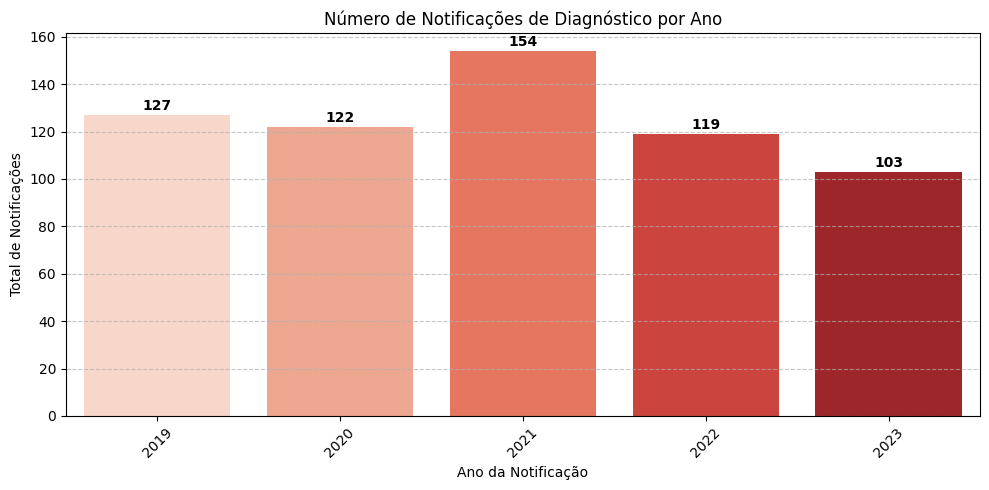
\includegraphics[width=1\linewidth]{imagens/NotificaçõesAno.png}
    \caption{Número de Gestantes com Sífilis Notificadas em Montes Claros e Seus Municípios Entre 2019 e 2023}
    \label{fig:enter-label}
\end{figure}

\begin{figure}[h!]
    \centering
    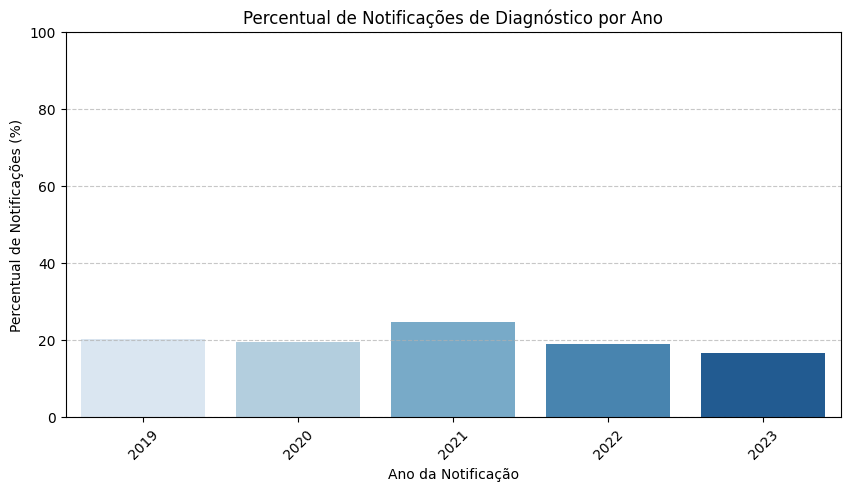
\includegraphics[width=1\linewidth]{imagens/Percentual_pelo_todo.png}
    \caption{Proporção de Gestantes com Sífilis Notificadas em Montes Claros e Seus Municípios Entre 2019 e 2023 em relação aos 5 Anos de Notificações}
    \label{fig:enter-label}
\end{figure}

Em 5 anos de coleta de dados, foram considerados 625 Gestantes com informações legivelmente fornecidas para a análise dos dados.
É possível evidênciar que em função dos 3 primeiros anos, houve um crescimento de aproximadamente 40 casos de sífilis em gestantes. Além de tudo nos últimos 3 anos houve um descrescimento gradual com mais de 45 casos de diferença entre 2021 e 2022, seguido de um descrescimento de aproximadamente 19 casos notificados de 2022 para 2023.

Observa-se mais detalhes sobre o comportamento em função dos anos no gráfico de proporção \textbf{Figura 2}.
\\
\\
\\

\subsubsection{Zonas de Residência}
\begin{figure}[h!]
    \centering
    \includegraphics[width=0.7\linewidth]imagens/{Residencia.png}
    \caption{Zona de Residências de Gestantes com Sífilis notificadas em Montes Claros e seus Municípios entre 2019 e 2023}
    \label{fig:enter-label}
\end{figure}

A proporção das gestantes notificadas com sífilis entre 2019 e 2023 se fez predominante em residentes de área urbana, de modo que em 2021 foi notificado um recorde de pelo menos 2\%, ou seja 4 das 167 gestantes notificadas com sífilis naquele ano eram residentes de zona rural.



\subsubsection{Raca das Gestantes}
\begin{figure}[h!]
    \centering
    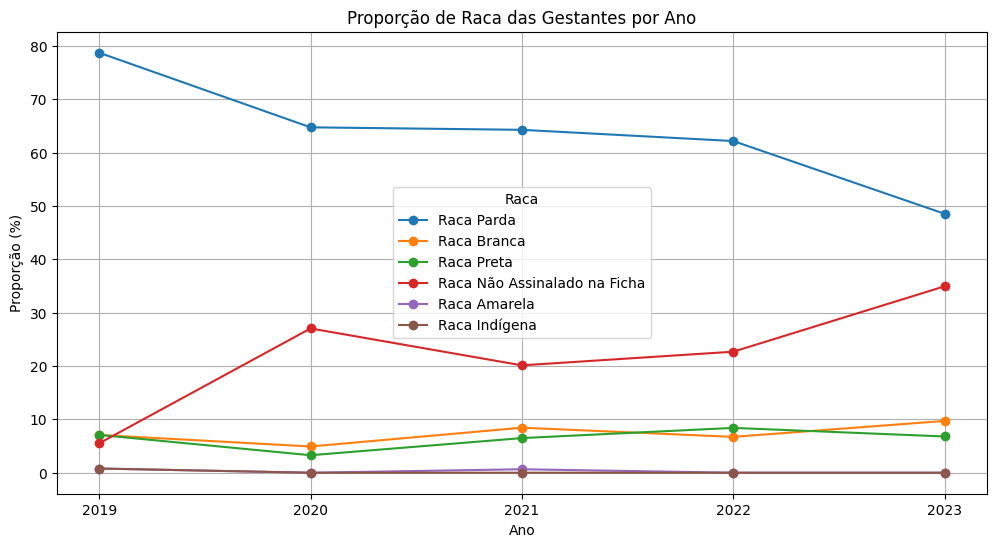
\includegraphics[width=0.7\linewidth]{imagens/RacaGestantes.png}
    \caption{Raca das Gestantes com Sífilis notificadas em Montes Claros e seus Municípios
entre 2019 e 2023}
    \label{fig:enter-label}
\end{figure}
A proporção das gestantes notificadas com sífilis entre 2019 e 2023 se fez predominante em gestantes de raça parda, de modo que em 2019 78.74\% das gestantes se identificavam como pardas e essa proporção foi diminuindo, de modo que em 2023 fosse de 48.54\%. Também é notório que, o número de gestantes que assinalaram a seção de ignorado na ficha de investigação cresceu de 5.51\% em 2019 para 34.95\% em 2023.

    Enquanto isso a menor proporção de gestantes que se identificam como brancas respondeu à ficha em 2020 representando 4.91\% da amostra.
    já a maior proporção de gestantes que se identificam como brancas respondeu à ficha em 2023 representando pelo menos 9.7\% da amostra.
    
    Ademais a menor proporção de gestantes que se identificam como pretas respondeu à ficha em 2020 representando 3.27\% da amostra.
    Para as que se identificaram como pretas, a maior proporção de gestantes que respondeu à ficha foi em 2022 representando 8.4\% da amostra.

    E gestantes que se identificavam como indígenas OU amarelas durante os 5 anos representavam sempre menos de 1\% da amostra.
    E gestantes que se identificavam como indígenas E as que se identificavam como amarelas durante os 5 anos somatizavam sempre menos de 1\% da amostra.

\subsubsection{Trimestre Gestacional da Notificação}
\begin{figure}[h!]
    \centering
    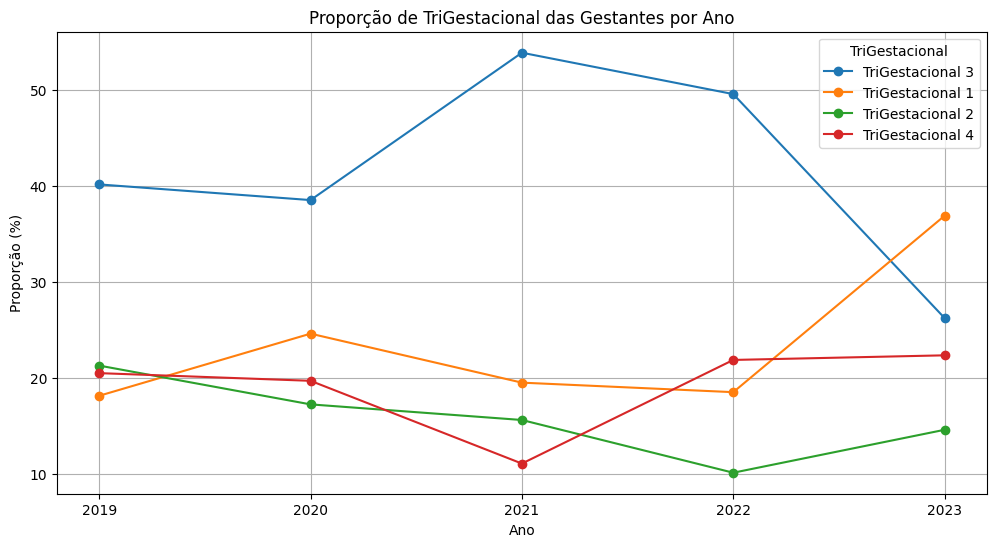
\includegraphics[width=0.7\linewidth]{imagens/TriGestacional.png}
    \caption{Trimestre Gestacional de Notificação das Gestantes com Sífilis em Montes Claros e seus Municípios entre 2019 e 2023}
    \label{fig:enter-label}
\end{figure}
 A proporção das gestantes notificadas com sífilis entre 2019 e 2023 se fez predominantemente quando as mesmas se encontravam no 3 trimestre gestacional até o ano de 2022. O número de gestantes notificadas no 1º Trimestre gestacional maior que as notificadas em outros períodos gestacionais.

Ademais poe-se perceber uma difícil notificação de gestantes no 2 trimestre gestacional, uma vez que esse número se representa menos de 20\% de todas as notificações em todos os anos.

Outra importante observação é que o menor número de notificações de gestantes notificadas no 4 período gestacional ocorreu em 2021 representando aproximadamente 10\% de todas as notificações do ano de 2021

É interessante observar que desde 2019 até 2023 o número de gestantes notificadas no 3º trimestre gestacional cairam de uma representação do todo de 40.42\% para 27.27\% . Enquanto isso as notificadas no 1º trimestre gestacional aumentaram de uma representação do todo de 18.43 \% para 33.76\%

Por fim observa-se que o pico em relação à outras notificações ocorreu em 2021, quando as notificações em relação ao todo de gestantes no 3º trimestre gestacional atingiram 55.54\%.
\\
\\
\subsubsection{Escolaridade das Gestantes}
\begin{figure}[h!]
    \centering
    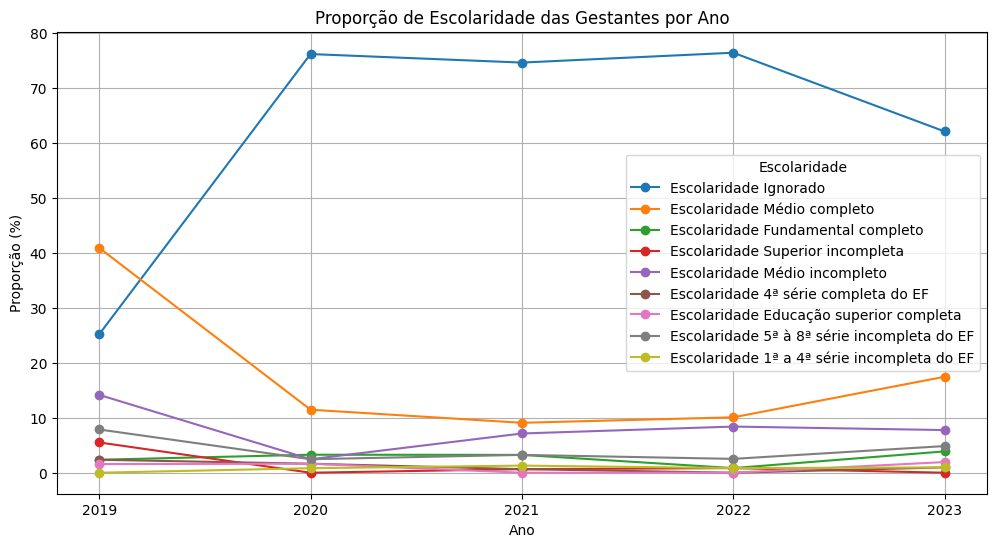
\includegraphics[width=0.7\linewidth]{imagens/Escolaridade.png}
    \caption{Escolaridade das Gestantes com Sífilis em Montes Claros e seus Municípios entre 2019 e 2023, das quais não ignoraram a seção de escolaridade}
    \label{fig:enter-label}
\end{figure}
 Das gestantes notificadas com sífilis entre 2019 e 2023 houve uma prevalência acima de 70\% que marcaram ignorado na seção escolaridade à partir de 2020. O ano onde menos houveram marcações nessa alternativa foi em 2019 com uma representação de 63.28\% do todo.

Sendo assim, das 625 gestantes, 230 não inoraram essa seção. Das 230 que assinalaram em 2019 54\% tinham apenas o ensino médio completo. Ademais, em 2022 35\% tinham o ensimo médio incompleto.
\begin{figure}[h!]
    \centering
    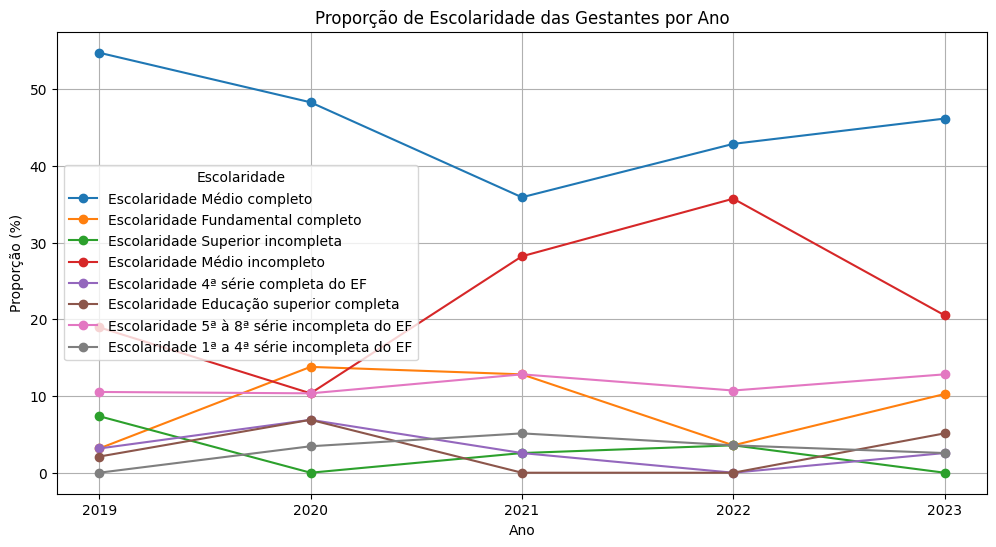
\includegraphics[width=0.7\linewidth]{imagens/EscolaridadeNãoIgnorada.png}
    \caption{Escolaridade das Gestantes com Sífilis em Montes Claros e seus Municípios entre 2019 e 2023, das quais não ignoraram a seção de escolaridade.}
    \label{fig:enter-label}
\end{figure}
\\
\\
\\
\\
\\
\\
\\
\\

\subsection{Análise de frequências e suas Distribuições}
Há uma notória concentração de notificações em Gestantes que dentre a amostragem analisada estão entre a faixa etária de 15 até 29 anos. De modo mais específico, a maioria das gestantes notificadas tem entre 15 e 24 anos.
\\
\begin{table}[h!]
\centering
\caption{Tabela de Frequência de Gestantes com Sífilis Notificadas em Montes Claros e seus Municípios entre 2019 e 2023}
\label{tab:frequencia_idades_intervalos}
\begin{tabular}{|c|c|c|}
\hline
Intervalo(Idade das Gestantes) & Frequência(Qtde. Neste Intervalo) & Porcentagem (\%) \\
\hline
10-14 & 6 & 0.96 \\
15-19 & 148 & 23.68 \\
20-24 & 244 & 39.04 \\
25-29 & 127 & 20.32 \\
30-34 & 53 & 8.48 \\
35-39 & 34 & 5.44 \\
40-44 & 12 & 1.92 \\
45-49 & 1 & 0.16 \\
\hline
\end{tabular}
\end{table}

\begin{figure}[h!]
    \centering
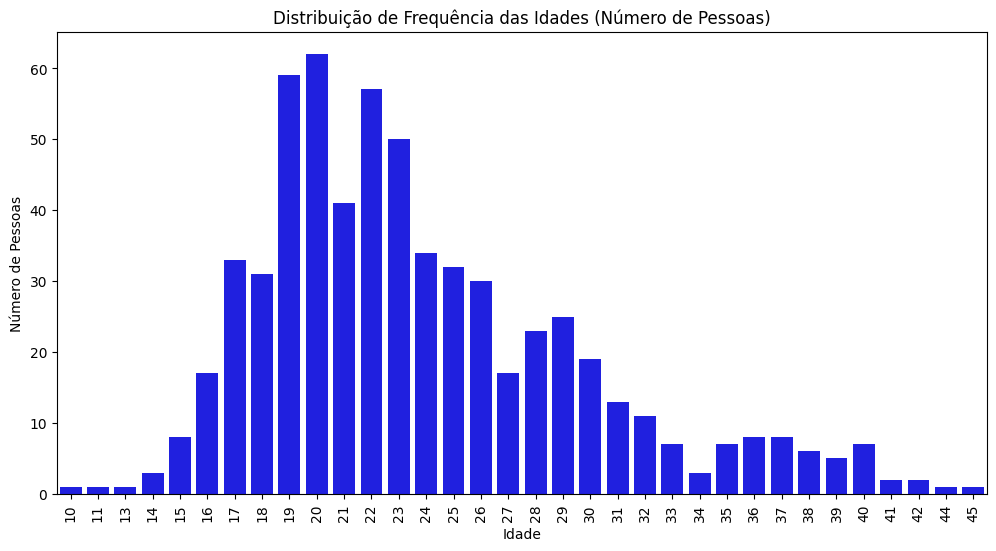
\includegraphics[width=0.7\linewidth]{imagens/FreqNums.png}
    \caption{Distribuição de Frequências sem Porcentagem das Gestantes}
    \label{fig:enter-label}
\end{figure}
\begin{figure}[h!]
    \centering
    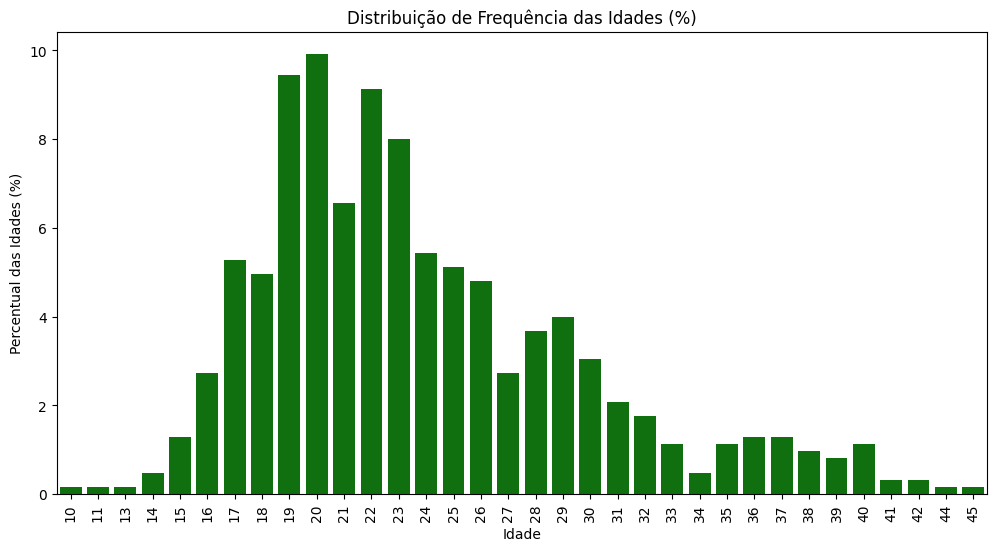
\includegraphics[width=0.7\linewidth]{imagens/FreqPercents.png}
    \caption{Distribuição de Frequências sem Porcentagem das Gestantes}
    \label{fig:enter-label}
\end{figure}

Ao realizar a elaboração de Box-Plots é possível visualizar máximos mínimos e como os quartis se comportam. Sendo assim, para idade e tratamento foi percebido que raras às exceções realizaram tratamento com \textit{Penicilina G benzantina 4 800 000 UI} acima dos 30 anos e nenhuma abaixo dos 17 anos. À fim de compreender melhor estes dados confira os demais boxplots abaixo:
\begin{figure}[h!]
    \centering
    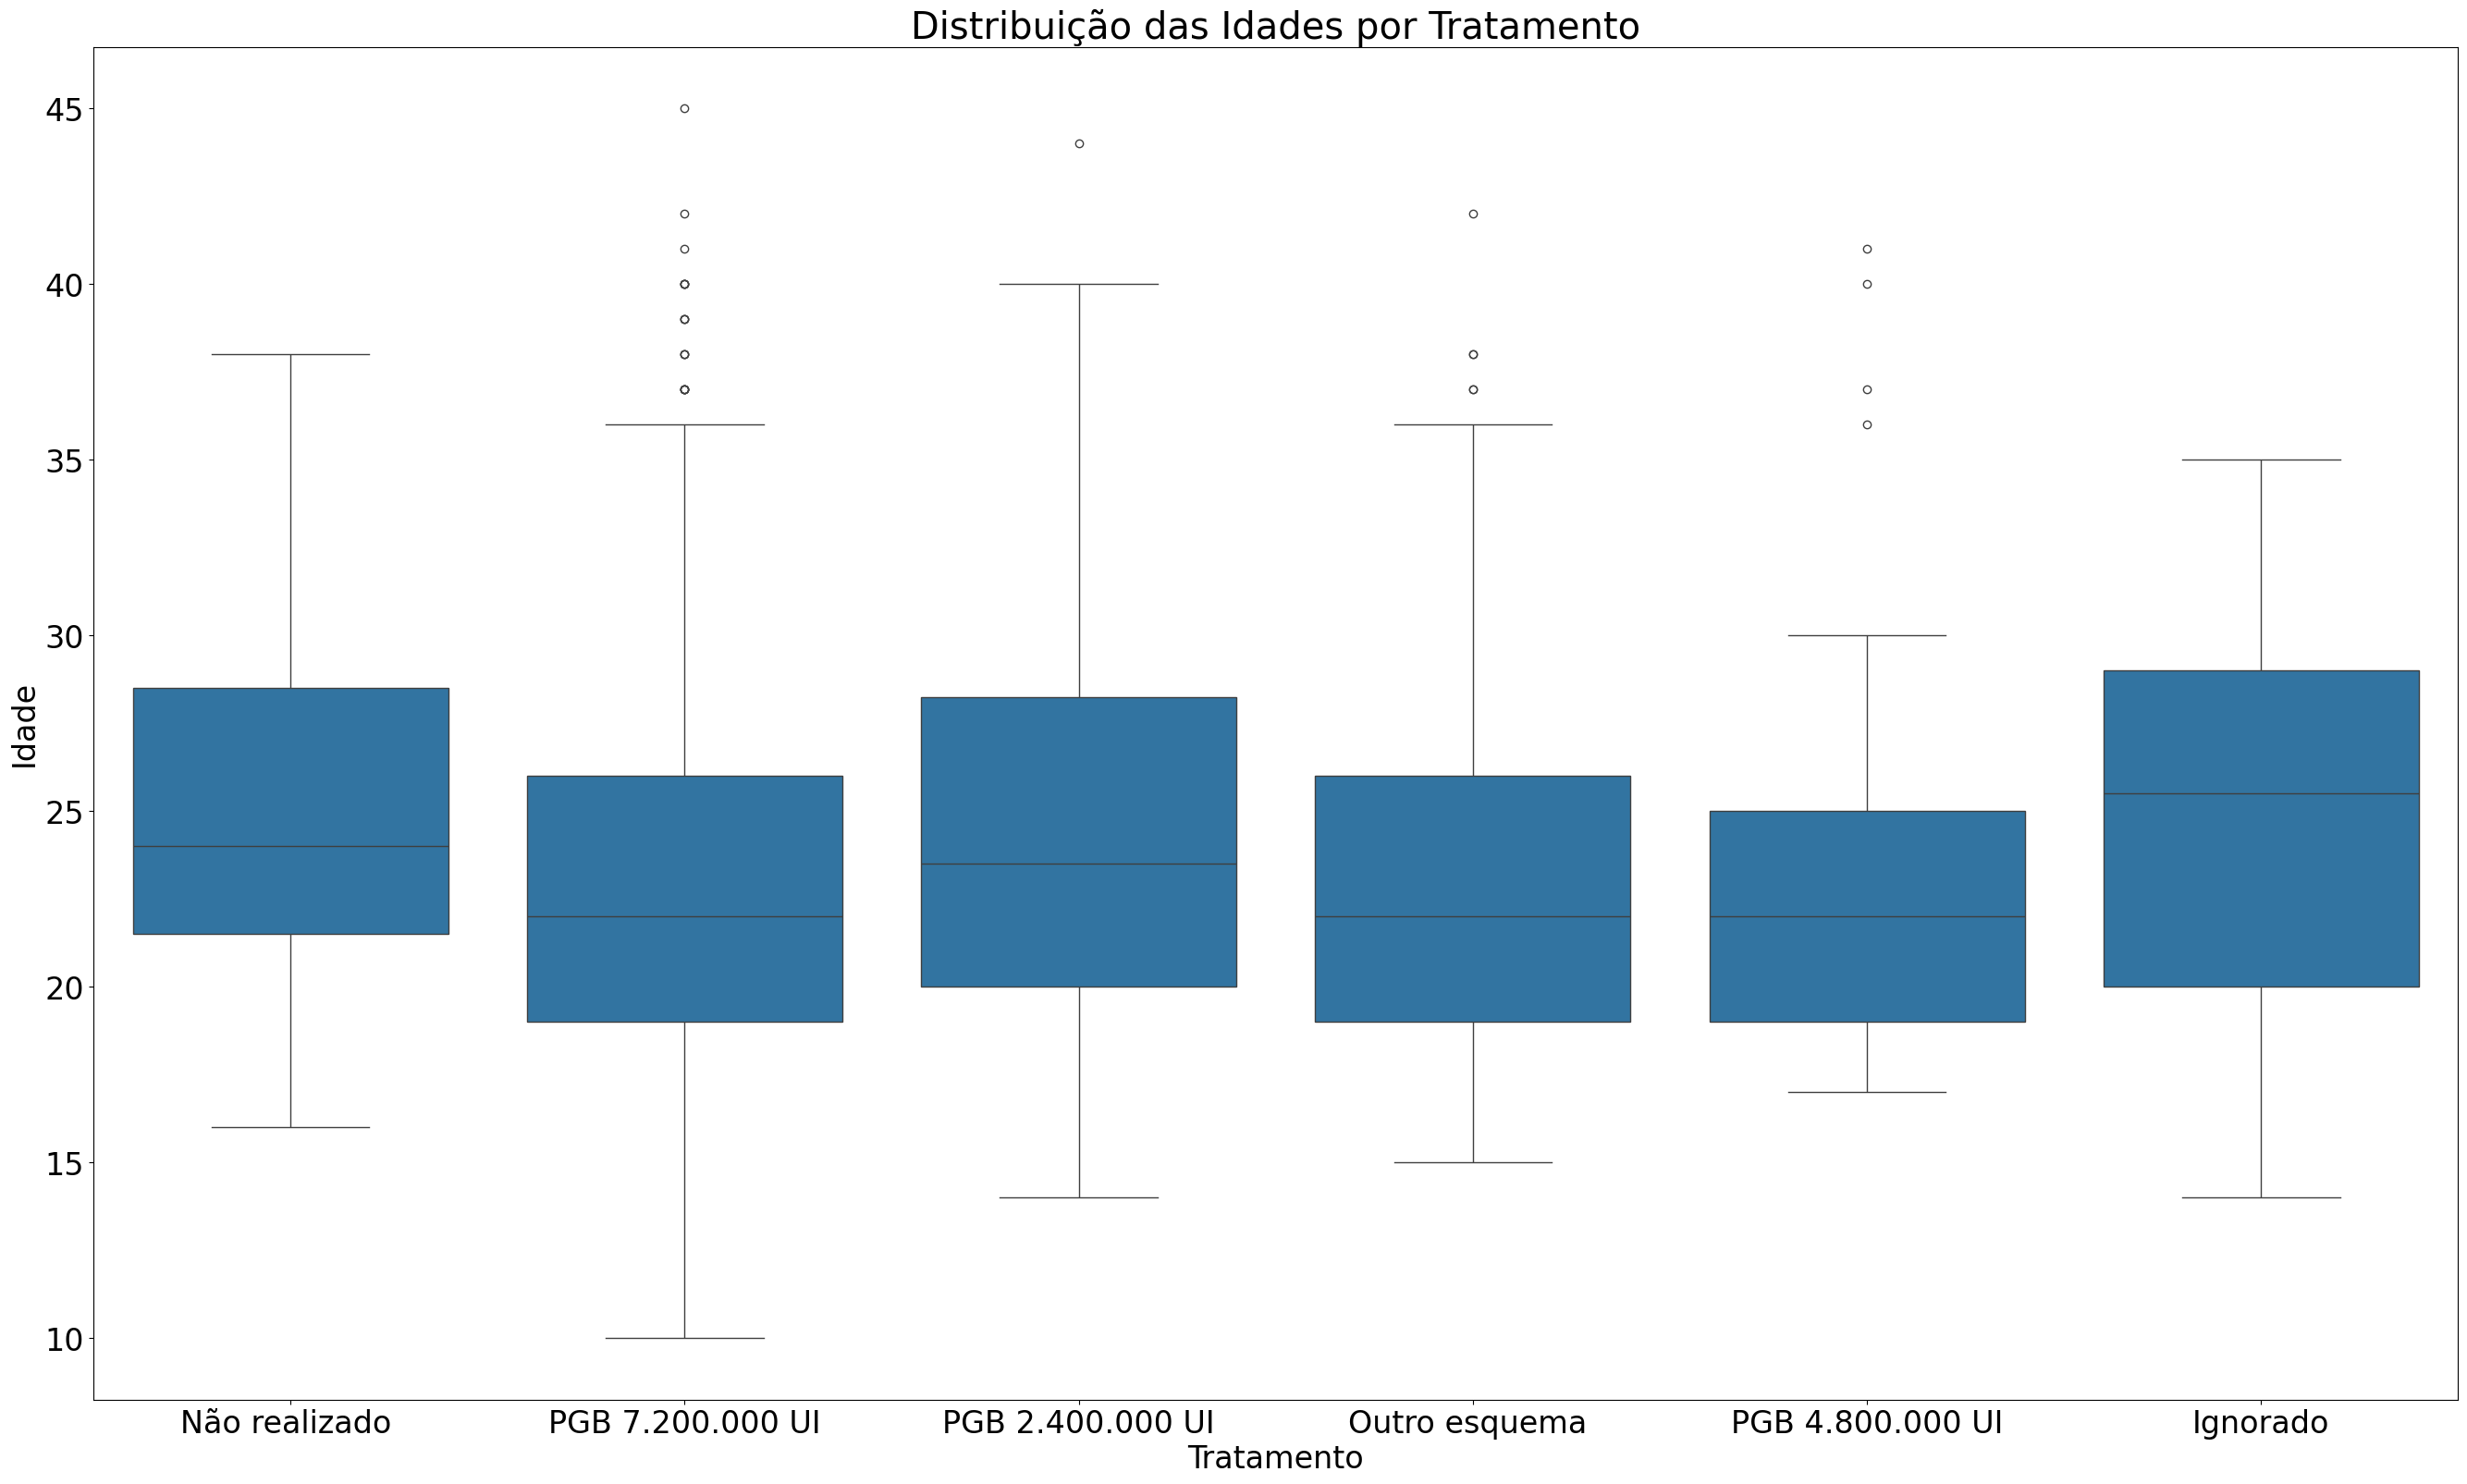
\includegraphics[width=1\linewidth]{imagens/tratamento_idade_boxplot.png}
    \caption{Distribuições das Idades por Tratamento}
    \label{fig:enter-label}
\end{figure}

\begin{figure}[h!]
    \centering
    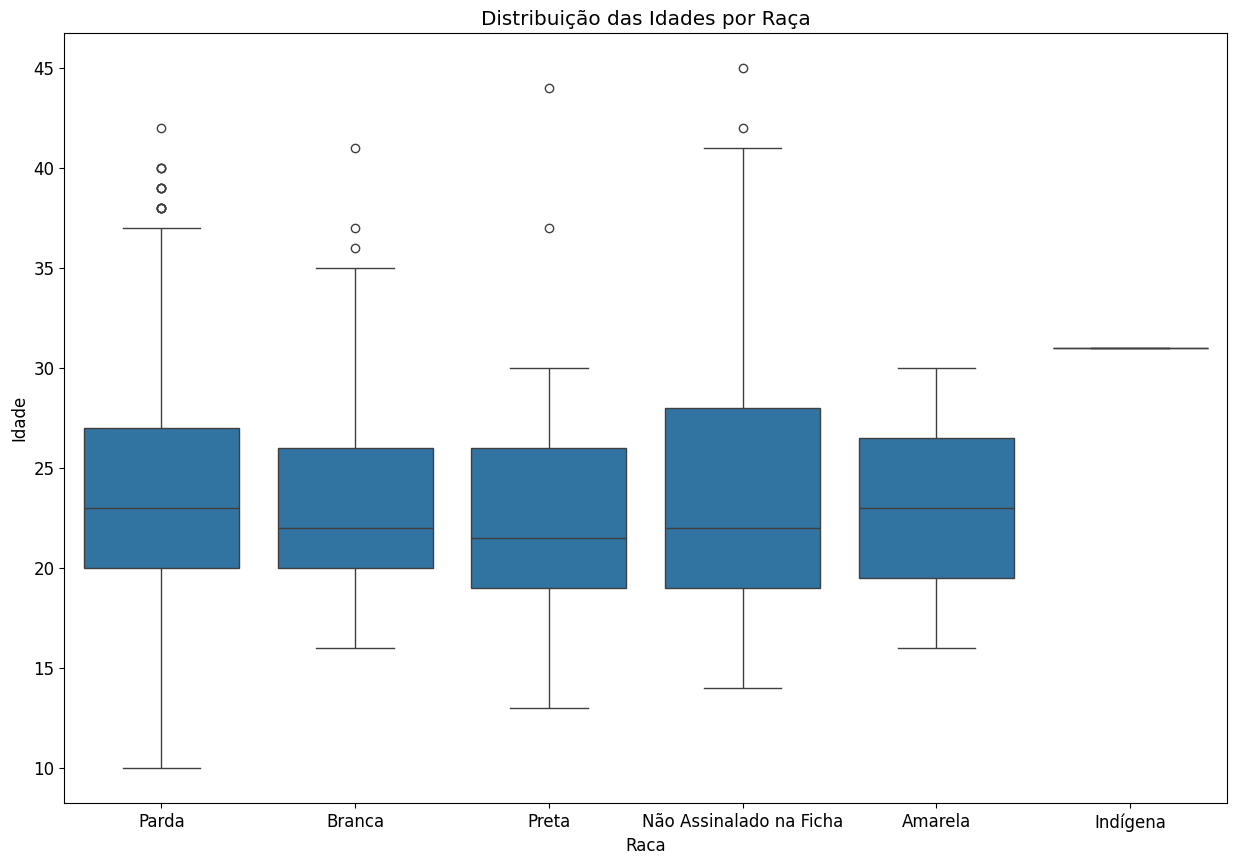
\includegraphics[width=1\linewidth]{imagens/Raca_idade_boxplot.png}
    \caption{Distribuições das Idades por Raça ou cor da pele}
    \label{fig:enter-label}
\end{figure}

\begin{figure}
    \centering
    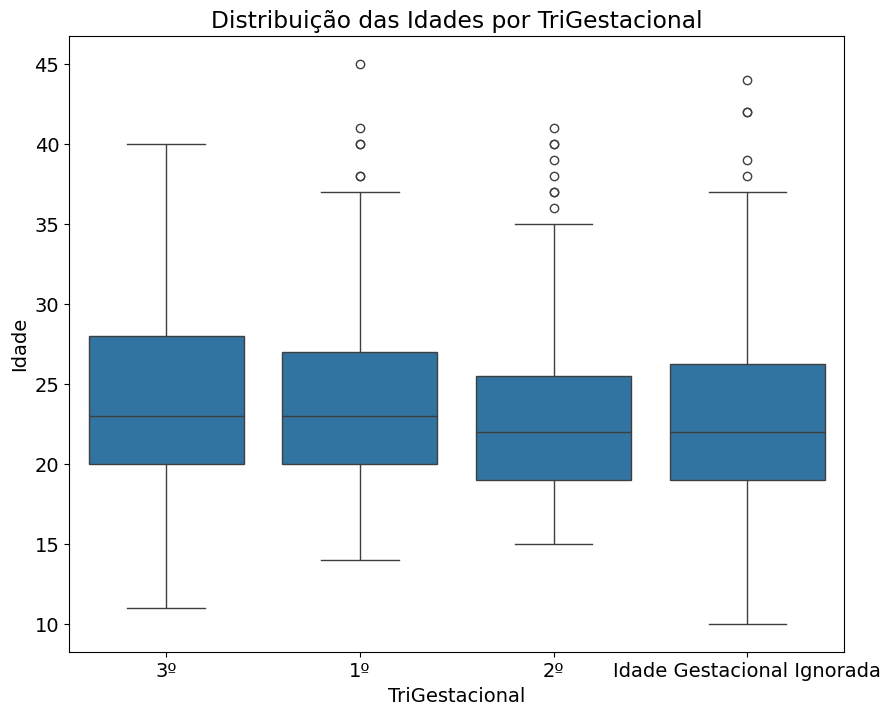
\includegraphics[width=1\linewidth]{imagens/TriGestacional_Idade_boxplot.png}
    \caption{Distribuições das Idades por Trimestres Gestacionais de Notificação}
    \label{fig:enter-label}
\end{figure}

\subsection{Investigando Associações Multivariadas}

\subsubsection{Gestantes Mais jovens são diagnosticadas mais tarde na gravidez?}

Teste de Kruskal-Wallis resultou em um p = 0.6133, indicando que não há diferença estatisticamente significativa nas medianas das idades entre os trimestres gestacionais. A idade das gestantes não varia significativamente entre os trimestres em que foram diagnosticadas.

Portanto, não é possível afirmar que: gestantes mais jovens são diagnosticadas mais tarde (ou mais cedo) na gravidez com base na base de dados analisada.


\subsubsection{Há uma associação entre a raça e o trimestre do diagnóstico?}
Os teste estatísticos levaram à comrpeensão de que há uma associação estatisticamente significativa entre raça e trimestre do diagnóstico gestacional, mas a força dessa associação é fraca (V de Cramer = 0.1170). Além disso, como a análise foi realizada desconsiderando as gestantes que marcaram 'ignorado' na ficha em sua subseção de raça, os resultados podem não ser totalmente representativos. Por isso, é importante continuar investigando outros fatores que possam influenciar o trimestre do diagnóstico.


\subsubsection{O tratamento difere para gestantes mais jovens em comparação às mais velhas?}
Foram realizados testes ANOVA e de Kruskal-Wallis, nestes não houveram evidências estatísticas para que o trataemnto fosse diferentes para gestantes jovens em comparação às mais velhas. Mais especificamente, a idade das gestantes não influencia significativamente o esquema de tratamento utilizado para a amostragem em questão.

\section{Conclusão}

\subsection{Perfil das Gestantes}
O perfil da gestante com sífilis entre 2019 e 2023 em Montes Claros e seus municípios é maior representado por pessoas entre 15 e 24 anos. Entre todas as gestantes de qualquer faixa etária, houveram majoritariamente mais notificações em 2019 e 2021. No que tange ao ensino das gestantes, mais de 60\% destas ignoraram a seção de escolaridade da ficha em todos os anos com excessão à 2019. Além de tudo, em todos os anos das que assinalaram a seção de escolaridade Escolaridade Média completa liderou em relação à proporção de outros níveis de escolaridade com mínimo de 37\% e máximo de 55\%. 

\subsection{Análise das Anomalias ou Outliers}
Perfis que são anormais ou não se enquadram nas gestantes também são analisados pelos boxplots.Dentre as amostras, gestantes que possuem mais de 38 anos e são notificadas até o 2º Trimestre Gestacional representam anormalidade no perfil de notificações realizadas. Ademais, Gestantes que se identificaram como raça preta acima de 30 anos também são consideradas anomalias na amostragem. 

A maior idade mínima de gestantes se prevaleceu entre as que se identificam de raça branca, e a menor idade mínima em pessoas que se identificam como pardas. Isso significa que gestantes entre 10 e 16 anos que se assumem como pardas não representam anormalidade na amostragem, mas gestantes definidas como brancas nessa mesma faixa etária sim são anormais ou outliers.

\subsection{Das perguntas Propostas}
Por fim, Não é possível que se estabeleça nenhuma das associações multivariadas propostas, uma vez que os dados não apresentam significativas associatividades ou discrepâncias de mediana entre colunas diferentes para que as hipóteses propostas sejam validadas ou rejeitadas estatísticamente.

\section{Referências}

\textbf{[1] AMORIM, E. K. R. et al.} Tendência dos casos de sífilis gestacional e congênita em Minas Gerais, 2009-2019: um estudo ecológico. Epidemiol. Serv. Saúde, v. 30, n. 4, p. e2021128, 2021. doi: 10.1590/S1679-49742021000400006.
\\\\
\textbf{[2] PAIXÃO, G. M. M. et al.} Machine Learning in Medicine: Review and Applicability. Arq Bras Cardiol, v. 118, n. 1, p. 95-102, jan. 2022. doi: 10.36660/abc.20200596.
\\\\
\textbf{[3] RAMESH, A. N. et al.} Artificial intelligence in medicine. Ann R Coll Surg Engl, v. 86, n. 5, p. 334-8, set. 2004. doi: 10.1308/147870804290.
\\\\
\textbf{[4] SOARES, K. K. S. et al.} Análise espacial da sífilis em gestantes e sífilis congênita no estado do Espírito Santo, 2011-2018. Epidemiol. Serv. Saúde, v. 29, n. 1, p. e2018193, 2020. doi: 10.5123/S1679-49742020000100018.
\\\\
\textbf{[5] Ministério da Saúde (Brasil).} Boletim Epidemiológico - Sífilis 2021. Número Especial / Out. 2021 Ano V - nº 01. Brasília, DF: Ministério da Saúde, 2021. Disponível em: https://www.gov.br/aids/pt-br/central-de-conteudo/boletins-epidemiologicos/2021/sifilis/bole\\tim\_sifilis\_2021\_internet.pdf/view. Acesso em: 22 fev. 2025.

\end{multicols}

\end{document}
